\documentclass[12pt,letterpaper]{article}
\usepackage[utf8]{inputenc}
\usepackage[spanish]{babel}
\usepackage{graphicx}
\usepackage[left=2cm,right=2cm,top=2cm,bottom=2cm]{geometry}
\usepackage{graphicx} % figuras
% \usepackage{subfigure} % subfiguras
\usepackage{float} % para usar [H]
\usepackage{amsmath}
%\usepackage{txfonts}
\usepackage{stackrel} 
\usepackage{multirow}
\usepackage{enumerate} % enumerados
\renewcommand{\labelitemi}{$-$}
\renewcommand{\labelitemii}{$\cdot$}
% \author{}
% \title{Caratula}
\begin{document}

% Fancy Header and Footer
% \usepackage{fancyhdr}
% \pagestyle{fancy}
% \cfoot{}
% \rfoot{\thepage}
%

% \usepackage[hidelinks]{hyperref} % CREA HYPERVINCULOS EN INDICE

% \author{}
\title{Caratula}

\begin{titlepage}
\begin{center}
\large{UNERSIDAD PRIVADA DE TACNA}\\
\vspace*{-0.025in}
\begin{figure}[htb]
\begin{center}

\includegraphics[width=8cm]{./Imagenes/logo}
\end{center}
\end{figure}
\vspace*{0.15in}
INGENIERIA DE SISTEMAS  \\

\vspace*{0.5in}
\begin{large}
TITULO:\\
\end{large}

\vspace*{0.1in}
\begin{Large}
\textbf{SESION DE LABORATORIO No  05 y 06} \\
\textbf{Administración de una Base de Datos Oracle} \\
\end{Large}

\vspace*{0.3in}
\begin{Large}
\textbf{CURSO:} \\
\end{Large}

\vspace*{0.1in}
\begin{large}
BASE DE DATOS II\\
\end{large}

\vspace*{0.3in}
\begin{Large}
\textbf{DOCENTE(ING):} \\
\end{Large}

\vspace*{0.1in}
\begin{large}
 Patrick Cuadros Quiroga\\
\end{large}

\vspace*{0.2in}
\vspace*{0.1in}
\begin{large}
Integrante: \\
\begin{flushleft}
Mamani Limache, Jhony 		\hfill	(2013046566) \\
Condori Tito, Hernan  		\hfill	(2009034553)  \\
Ordoñez Quilli, Ronald		\hfill	(2015052821) \\
Moreno Caceres, Renzo Alex	\hfill	(2013047246)\\
Zavala Venegas, Luis Angel	\hfill	(2010037899)\\
Condori Quiso, Jesus		\hfill	(2008032440)
\end{flushleft}
\end{large}
\end{center}

\end{titlepage}


\tableofcontents % INDICE
\thispagestyle{empty} % INDICE SIN NUMERO
\newpage
\setcounter{page}{1} % REINICIAR CONTADOR DE PAGINAS DESPUES DEL INDICE


\section{Laboratorio No 05 – Cuestionario} 

\begin{enumerate}[1.]
	\item Los valores introducidos al archivo sysctl.conf ¿que representan?
	\begin{center}
	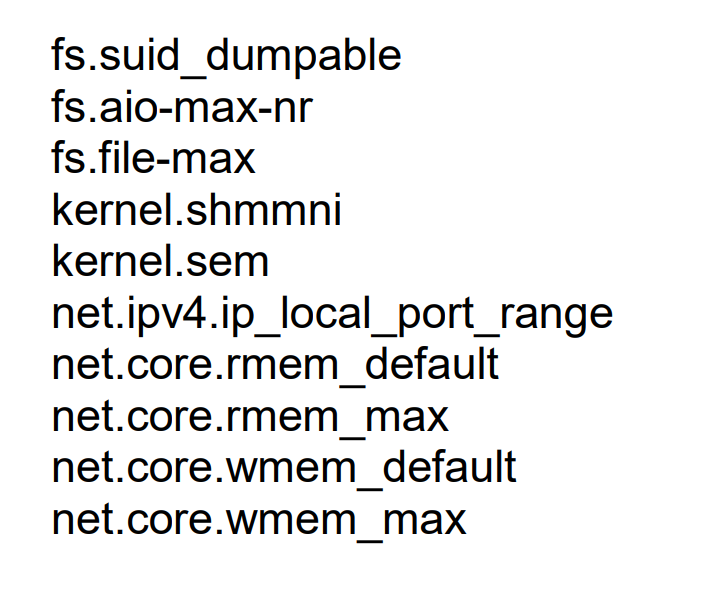
\includegraphics[width=8cm]{./Imagenes/actividad_5_1_lab_05}
	\end{center}
	\item ¿Con qué usuario(s) puedo conectarme al servidor a través del Administrador Empresarial?
	\\
	\\ se podra ingresar con 2 grupos de usuarios oinstall y dba, así como una cuenta de usuario llamada oracle

	\item Capture una imagen de pantalla del navegador con el Administrador Empresarial, con el nombre de su servidor e iniciada la sesión del usuario SYS.

	\begin{center}
	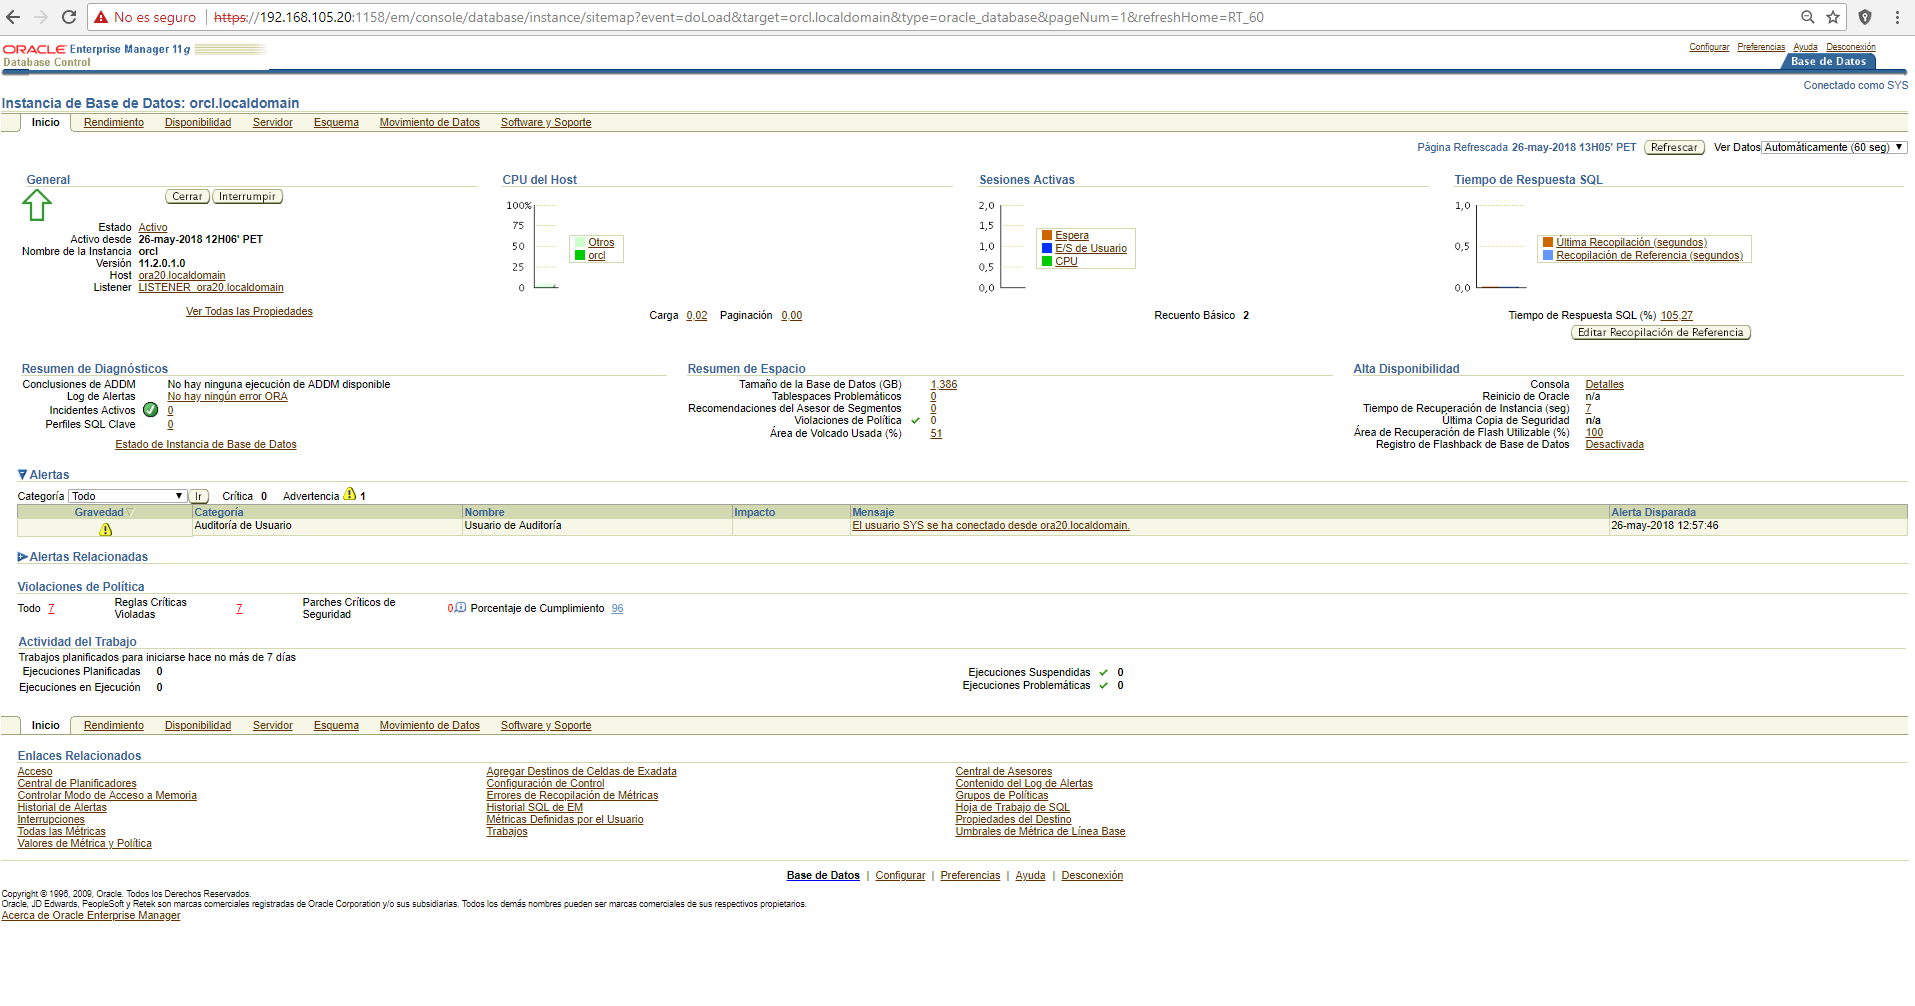
\includegraphics[width=15cm]{./Imagenes/Lab5-5_3} 
	\end{center}
	
	

\end{enumerate} 

\section{Actividad No 02 – Cuestionario} 

\begin{enumerate}[1.]
	\item ¿Qué sucede al ejecutar los siguientes comandos?

	\item . En el script lab\_02\_01.sql, se establecen privilegios de sistema, enliste los privilegios de sistema (DDL) utilizados y describa cada uno de ellos.
	
	\item Enliste y describa los tipos de TableSpace que existen en Oracle.
	
	

\end{enumerate} 

\section{Laboratorio No 07 – Cuestionario} 

\begin{enumerate}[1.]
	
	\item Desarrollar el scrip de creaci\'on de TableSpace y archivos para la base de datos de su proyecto.
	\\Conectarse con SQL Developer

	\begin{center}
	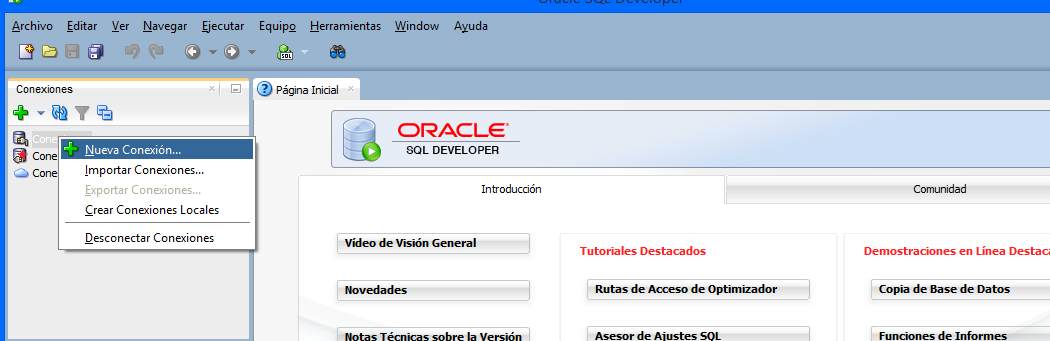
\includegraphics[width=8cm]{./Imagenes/eje7_con}
	\end{center}	
	coloque un nombre de conexi\'on, el usuario es system y la contraseña es 123456, system es un usuario administrador, por defecto sqldeveloper coloca el SID como XE, modif\'iquelo por el nombre Oracle
	\\Conectar y entrar\'a el area de trabajo de SQL Developer

	\begin{center}
	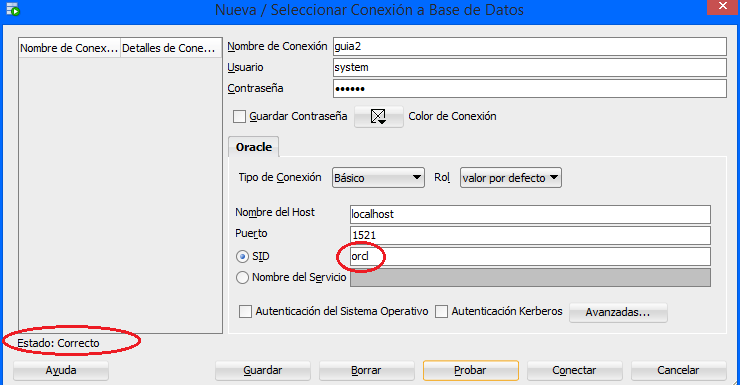
\includegraphics[width=8cm]{./Imagenes/eje_con1}
	\end{center}	

	Digite las sentencias para crear la tabla G2 e insertar los datos\\
	\begin{center}
	\includegraphics[width=8cm]{./Imagenes/eje_con2}
	\end{center}	
	Realice pruebas con los comandos vistos en Base de datos I, UPDATE, DELETE, SELECT y podr\'a comprobar que el lenguaje de manipulaci\'on de datos(DML), se mantiene similar al de SQL Server e incluso con MySql\\
	\begin{center}
	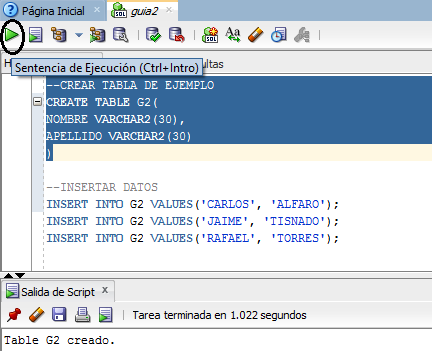
\includegraphics[width=8cm]{./Imagenes/eje_con3}
	\end{center}	
	\item Desarrollar el scrip de creaci\'on de objetos (entidades, atributos, llaves y rectriccion
	\\Conectarse con SQL PLUS
	\begin{center}
	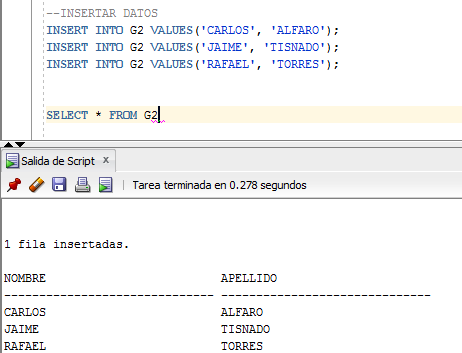
\includegraphics[width=8cm]{./Imagenes/eje1}
	\end{center}	
	Para comenzar muestre los datos de la tabla g2, creada en SQL Developer, debe mostrar los siguientes datos, si no aparecen datos significa que no ejecut\'o la sentencia commit\\
	\begin{center}
	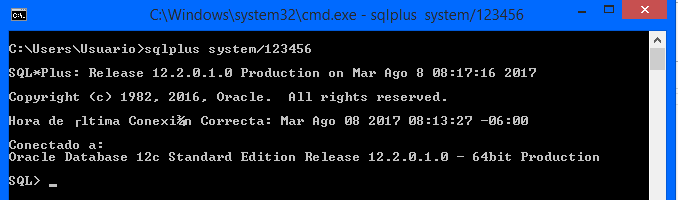
\includegraphics[width=8cm]{./Imagenes/eje2}
	\end{center}	
	Procedemos a crear la tabla g3, es importante verificar que cuando tenemos una sentencia de una sola l\'inea como (select * from g2)\\
	\begin{center}
	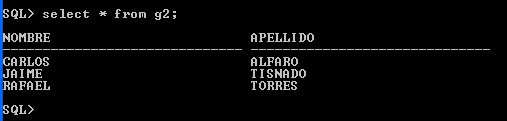
\includegraphics[width=8cm]{./Imagenes/eje3}
	\end{center}	
	Agregue los siguientes registros y realice modificaciones y eliminaciones\\
	\begin{center}
	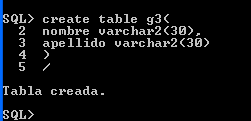
\includegraphics[width=8cm]{./Imagenes/eje4}
	\end{center}	
	Si deseamos conocer la estructura que tiene una tabla podemos utilizar la sentencia DESC TABLE\\
	\begin{center}
	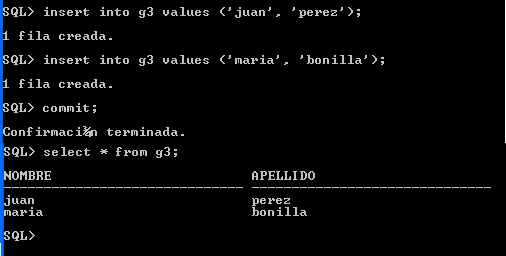
\includegraphics[width=8cm]{./Imagenes/eje5}
	\end{center}
	CREACION DE USUARIOS Y TABLESPACE
	En la unidad D, cree una carpeta que se llame prueba
	Digite el siguiente c\'odigo, que permitir\'a crear un table espace de 32 mb en la carpeta prueba de la unidad D\\
	\begin{center}
	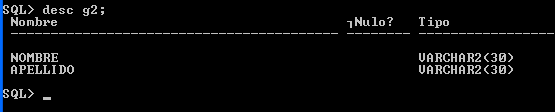
\includegraphics[width=8cm]{./Imagenes/eje6}
	\end{center}
	Ahora crearemos un usuario llamado udbg2 con clave don bosco y en la siguiente l\'inea le asignaremos permisos de administrador( grant dba to 		udbg2)\\
	\begin{center}
	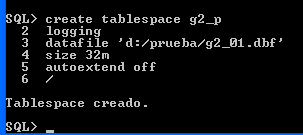
\includegraphics[width=8cm]{./Imagenes/eje7}
	\end{center}
	Ahora si necesidad de salirnos de SQL PLUS podemos cambiarnos de usuarios con la sentencia connect user/clave, luego podemos verificar el usuario actual con la consulta select user from dual, tambi\'en puede utilizar la sentencia show user\\
	\begin{center}
	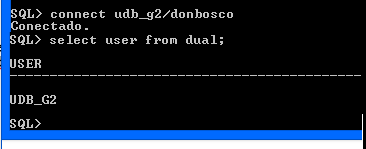
\includegraphics[width=8cm]{./Imagenes/eje8}
	\end{center}
	En el usuario UDBG2 crearemos las siguientes tablas\\
	\begin{center}
	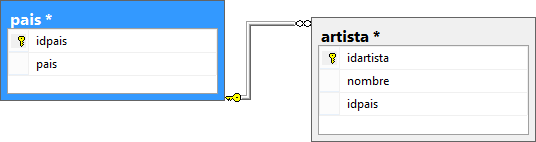
\includegraphics[width=8cm]{./Imagenes/eje9}
	\end{center}
	\begin{center}
	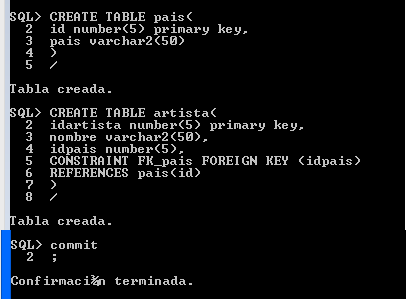
\includegraphics[width=8cm]{./Imagenes/eje10}
	\end{center}
	Para verificar si las tablas fueron creadas podemos utilizar la siguiente sentencia\\
	\begin{center}
	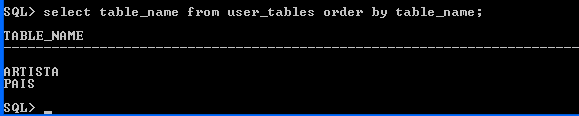
\includegraphics[width=8cm]{./Imagenes/eje11}
	\end{center}
	Finalmente insertamos los datos de la tabla pa\'is y artista\\
	\begin{center}
	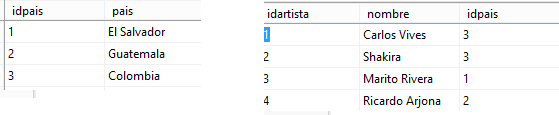
\includegraphics[width=8cm]{./Imagenes/eje12}
	\end{center}
	ANALISIS DE RESULTADOS
	Crear un tablespace con el nombre de ejercicio1 y crear un usuario con su c\'odigo de carnet, a dicho usuario asignar el tablespace y crear las 		siguientes tablas\\
	\begin{center}
	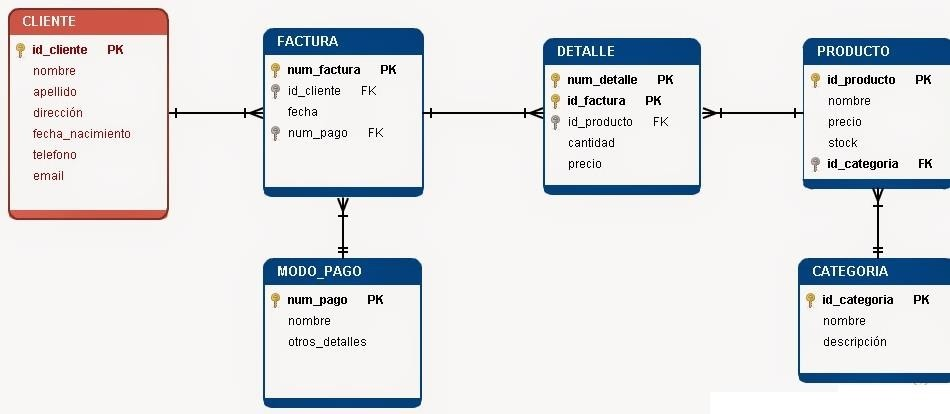
\includegraphics[width=8cm]{./Imagenes/eje13}
	\end{center}
\end{enumerate} 





\end{document}
